\documentclass[tikz, border=10pt]{standalone}
\usetikzlibrary{arrows.meta, positioning, shapes, calc}

\usepackage[T1]{fontenc}
\usepackage{lmodern}
\begin{document}
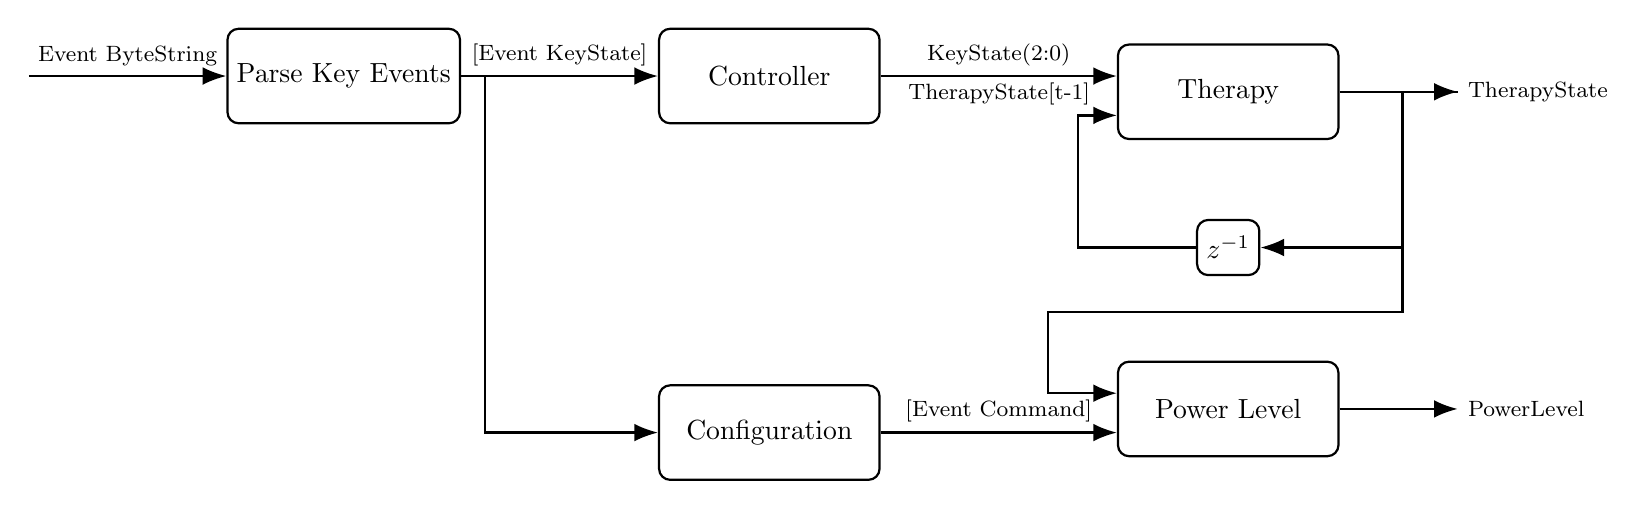
\begin{tikzpicture}[
  block/.style = {draw, thick, minimum width=2.8cm, minimum height=1.2cm, align=center, rounded corners},
  sum/.style = {draw, circle, inner sep=1pt, minimum size=6mm, node contents={+}},
  line/.style = {thick, -{Latex[length=3mm]}},
  signal/.style = {font=\footnotesize, midway, above},
  signalbelow/.style = {font=\footnotesize, midway, below}
]

  % Nodes
  \node[block] (parser) {Parse Key Events};
  \node[block, right=2.5cm of parser] (controller) {Controller};
  \node[block, right=3cm of controller, yshift=-0.2cm] (therapy) {Therapy};
  \node[block, minimum size=7mm, below=1cm of therapy] (delay) {$z^{-1}$};
  \node[block, below=3.3cm of controller] (configuration) {Configuration};
  \node[block, right=3cm of configuration, yshift=0.3cm] (powerlevel) {Power Level};

  % Connections
  \draw[line] (-4,0) -- (parser.west) node[signal]{Event ByteString};
  \draw[line] (parser.east) -- node[signal]{[Event KeyState]} (controller.west);

  % Controller to Therapy
  \draw[line] (controller.east) -- node[signal]{KeyState(2:0)} ([yshift=0.2cm]therapy.west);

  % Therapy output
  \draw[line] (therapy.east) -- ++(1.5,0) coordinate (out) node[right, font=\footnotesize]{TherapyState};

  % Feedback path through delay
  \draw[line] (out) -- ++(-0.7,0)|- (delay.east);
  \draw[line] (delay.west) -| ++(-1.5,1.5) |- ([yshift=-0.3cm]therapy.west) node[signal, above, xshift=-1cm]{TherapyState[t-1]};

  % Stage 2
  \draw[line] ([xshift=1cm]parser.east) -- ++(-0.7,0)|- (configuration.west);
  \draw[line] (configuration.east) -- node[signal]{[Event Command]} ([yshift=-0.3cm]powerlevel.west);
  \draw[line] ([xshift=-0.7cm]out) -- ++(0,-2.8) |- ++(-4.5,0) |- ([yshift=0.2cm]powerlevel.west);
  \draw[line] (powerlevel.east) -- ++(1.5,0) node[right, font=\footnotesize]{PowerLevel};

\end{tikzpicture}
\end{document}
